\documentclass{article}
\usepackage[utf8]{inputenc}
\setlength{\parskip}{5pt} % esp. entre parrafos
\setlength{\parindent}{0pt} % esp. al inicio de un parrafo
\usepackage{listings} % listings
\usepackage{color} %colores
\usepackage{amsmath} % mates
\usepackage[sort&compress,numbers]{natbib} % referencias
\usepackage{url} % que las URLs se vean lindos
\usepackage[top=15mm,left=20mm,right=20mm,bottom=25mm]{geometry} % margenes
\usepackage{hyperref} % ligas de URLs
\usepackage{graphicx} % poner figuras
\usepackage[spanish,es-tabla]{babel} % nombre tablas
\usepackage{caption}
\usepackage{subcaption}



\definecolor{mypink}{rgb}{0.976, 0.462, 0.847}
\definecolor{mygray}{rgb}{0.976, 0.980, 0.980}
\definecolor{myblue}{rgb}{0.258, 0.682, 1}
\definecolor{mypink2}{rgb}{0.525, 0.054, 0.4}
\lstset{ 
  backgroundcolor=\color{mygray},
  commentstyle=\color{myblue},
  keywordstyle=\color{mypink}, 
  numberstyle=\tiny\color{mypink}
  stringstyle=\color{mypink2}, 
  breaklines=true,
}

\title{Tarea 10}
\author{Eduardo Navarro}
\date{Noviembre 2021}

\begin{document}

\maketitle

\section{Introducción}
En esta práctica se evaluaron las instancias a diferentes reglas para el problema de la mochila en donde se observaron resultados interesantes para diferentes casos.

\section{Desarrollo}
Con las instrucciones de la tarea \cite{algenetic} y lo visto en clase \cite{twitchsimu} se le hicieron modificaciones al código para obtener las reglas \cite{maria} y evaluar a un tiempo determinado \cite{contador}. Así mismo se añadió un \texttt{for} para hacer las repeticiones y otro \texttt{for} para las instancias para cada una de las reglas. Posteriormente se realizó el correspondiente análisis estadístico.

\begin{lstlisting} [language=R, caption= Código para las reglas.]
#Modificacion para la regla 1
generador.pesos <- function(cuantos, min, max) {
  return(sort(round(runif(cuantos) * (max - min) + min)))
}

generador.valores <- function(cuantos, min, max) {
  return(round(runif(cuantos) * (max - min) + min))
}

#Modificacion para la regla 2
generador.pesos <- function(valores, min, max) {
  n <- length(valores)
  pesos <- double()
  for (i in 1:n) {
    media <- valores[i]
    desv <- runif(1, max=.1)
    ruido <- rnorm(1, sd=.1)
    pesos <- c(pesos, rnorm(1, (1/media), desv) + ruido)
  }
  pesos <- normalizar(pesos) * (max - min) + min
  return(pesos)
}

generador.valores <- function(cuantos, min, max) {
  return(sort(round(normalizar(rexp(cuantos)) * (max - min) + min)))
}

    n <- 50
    pesos <- generador.pesos(valores, 15, 80)
    valores <- generador.valores(n, 10, 500)
    capacidad <- round(sum(pesos) * 0.65)

#Modificacion para la regla 3
generador.pesos <- function(cuantos, min, max) {
  return(sort(round(normalizar(rnorm(cuantos)) * (max - min) + min)))
}

generador.valores <- function(pesos, min, max) {
  n <- length(pesos)
  valores <- double()
  for (i in 1:n) {
    media <- pesos[i]
    desv <- runif(1)
    ruido <- rnorm(1, sd=.1)
    valores <- c(valores, rnorm(1, media^2, desv) + ruido)
  }
  valores <- normalizar(valores) * (max - min) + min
  return(valores)
}
\end{lstlisting}

Para cada regla se agregó la probabilidad de mutación, cantidad de cruzamiento y tamaño de población a distintos valores dejando los otros 2 constantes a los cuales se le incluyeron réplicas.

\begin{lstlisting} [language=R, caption= Código para las instancias.]

#probabilidad de mutacion
pmutant<-c(0.05,0.1,0.5)
j<- 1:3
for (pm in pmutant){
for (replicas in j){

n <- 50
pesos <- generador.pesos(n, 15, 80)
valores <- generador.valores(pesos, 10, 500)
capacidad <- round(sum(pesos) * 0.65)
optimo <- knapsack(capacidad, pesos, valores)
init <- 30
p <- poblacion.inicial(n, init)
tam <- dim(p)[1]
assert(tam == init)

rep <- 10


#cantidad de cruzamiento
reproducc<-c(10, 20, 30)
j<- 1:3
for (rep in reproducc){
for (replicas in j){

n <- 50
pesos <- generador.pesos(n, 15, 80)
valores <- generador.valores(pesos, 10, 500)
capacidad <- round(sum(pesos) * 0.65)
optimo <- knapsack(capacidad, pesos, valores)
init <- 30
p <- poblacion.inicial(n, init)
tam <- dim(p)[1]
assert(tam == init)
pm <- 0.05

#tamano de poblacion
poblacion<-c(20, 30, 40)
j<- 1:3
for (init in poblacion){
for (replicas in j){

n <- 50
pesos <- generador.pesos(n, 15, 80)
valores <- generador.valores(pesos, 10, 500)
capacidad <- round(sum(pesos) * 0.65)
optimo <- knapsack(capacidad, pesos, valores)

p <- poblacion.inicial(n, init)
tam <- dim(p)[1]
assert(tam == init)
pm <- 0.05
rep <- 10
\end{lstlisting}

Para su evaluación se cambiaron las iteraciones por un límite de tiempo que se agregó con un \texttt{while} a 5 segundos.

\begin{lstlisting} [language=R, caption= Código para el límite de tiempo.]
mejores <- double()

timer = 5
start = Sys.time()

while(TRUE) {
  elapsed = as.numeric(difftime(Sys.time(), start, units = 'secs'))
  remaining = timer - round(elapsed) 
  Sys.sleep(.1)
  
  print(remaining)

  p$obj <- NULL
  p$fact <- NULL
  ....
  print(paste(mejor, (optimo - mejor) / optimo))
  
  
  faltaaloptimo<-(optimo - mejor) / optimo
  segundos<-round(elapsed)
  
  if (remaining <= 0) break
\end{lstlisting}

Se capturó todo en un \texttt{data.frame} respectivo para cada regla con cada instancia.

\begin{lstlisting} [language=R, caption= Ejemplo de código para el \texttt{data.frame}.]
datos = data.frame()

pmutant<-c(0.05,0.1,0.5)
j<- 1:3
....
  faltaaloptimo<-(optimo - mejor) / optimo
  segundos<-round(elapsed)

  if (remaining <= 0) break
  
  
  resultado = c(replicas, segundos, mejor,faltaaloptimo,pm,optimo)
  datos = rbind(datos, resultado)
  names(datos) = c("replicas", "segundo", "mejor", "%optimo", "pm","Optimo")
}
\end{lstlisting}

Después de la aplicación de una regla los siguientes valores se analizaron manteniendo el mismo entorno al correr el programa a partir del último \texttt{data.frame}. A partir del programa se obtuvo una tabla \ref{tabla1}.

\begin{table}[h!]
\centering
\caption{Ejemplo de datos obtenidos.}
\label{tabla1}
\begin{tabular}{|c|c|r|r|r|r|}
\hline
\textbf{replicas} & \textbf{segundo} & \multicolumn{1}{c|}{\textbf{mejor}} & \multicolumn{1}{c|}{\textbf{\%optimo}} & \multicolumn{1}{c|}{\textbf{pm}} & \multicolumn{1}{c|}{\textbf{Optimo}} \\ \hline
1 & 0 & 9341 & 0.194811 & 0.05 & 11601 \\ \hline
1 & 1 & 9341 & 0.194811 & 0.05 & 11601 \\ \hline
1 & 1 & 9341 & 0.194811 & 0.05 & 11601 \\ \hline
1 & 2 & 9475 & 0.183260 & 0.05 & 11601 \\ \hline
\end{tabular}
\end{table}

Con los datos de la tabla que se generan para cada regla en cada una de las instancias se procedió a graficar primero para la regla 1. 

\begin{figure}[h!]
\centering
\caption{Variación de probabilidad de mutación para la regla 1.}
\begin{subfigure}[b]{0.3\linewidth}
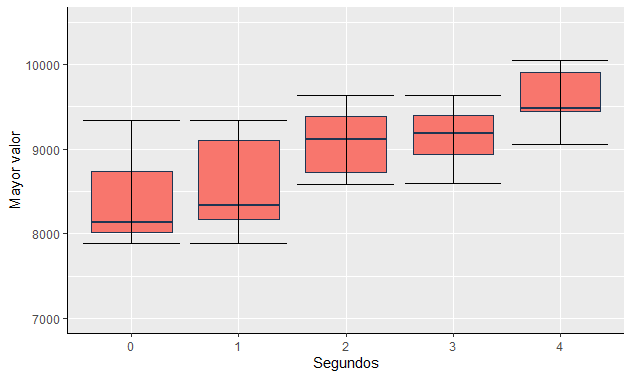
\includegraphics[width=\linewidth]{r1pm0.05.png}
\caption{0.05}
\label{am1}
\end{subfigure}
\begin{subfigure}[b]{0.3\linewidth}
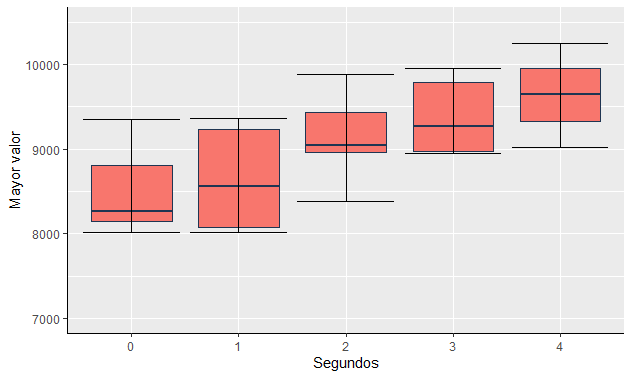
\includegraphics[width=\linewidth]{r1pm0.1.png}
\caption{0.1}
\label{bm1}
\end{subfigure}
\begin{subfigure}[b]{0.3\linewidth}
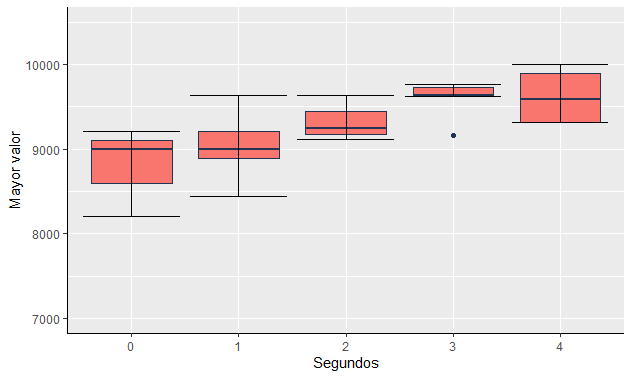
\includegraphics[width=\linewidth]{r1pm0.5.png}
\caption{0.5}
\label{cm1}
\end{subfigure}
\label{fig1}
\end{figure}

\begin{figure}[h!]
\centering
\caption{Variación de cruzamientos para la regla 1.}
\begin{subfigure}[b]{0.3\linewidth}
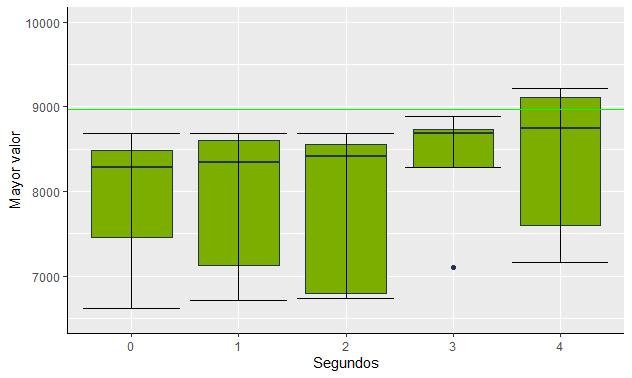
\includegraphics[width=\linewidth]{r1rep10.png}
\caption{10}
\label{ac1}
\end{subfigure}
\begin{subfigure}[b]{0.3\linewidth}
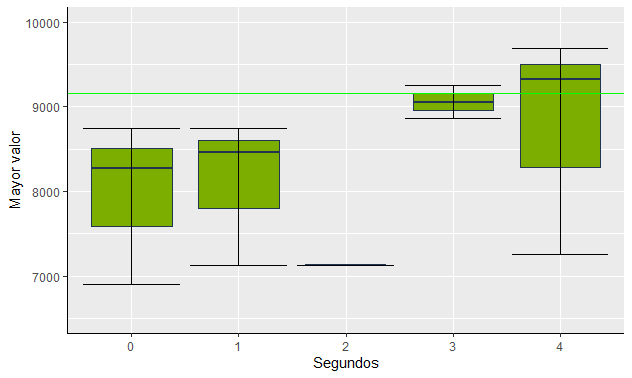
\includegraphics[width=\linewidth]{r1rep20.png}
\caption{20}
\label{bc1}
\end{subfigure}
\begin{subfigure}[b]{0.3\linewidth}
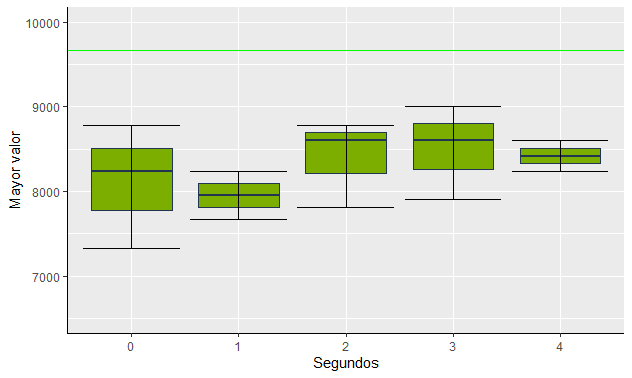
\includegraphics[width=\linewidth]{r1rep30.png}
\caption{30}
\label{cc1}
\end{subfigure}
\label{fig2}
\end{figure}

\newpage

\begin{figure}[h!]
\centering
\caption{Variación de población para regla 1.}
\begin{subfigure}[b]{0.3\linewidth}
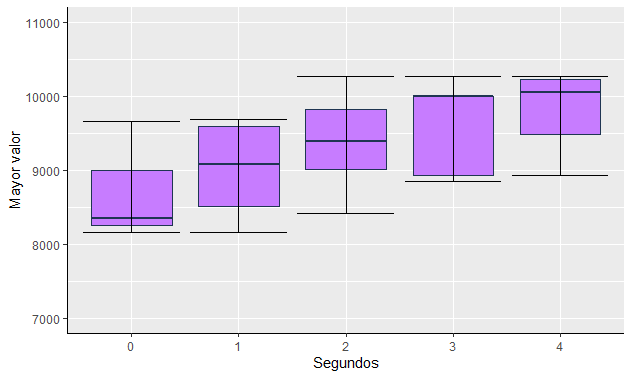
\includegraphics[width=\linewidth]{r1pob20.png}
\caption{20}
\label{ap1}
\end{subfigure}
\begin{subfigure}[b]{0.3\linewidth}
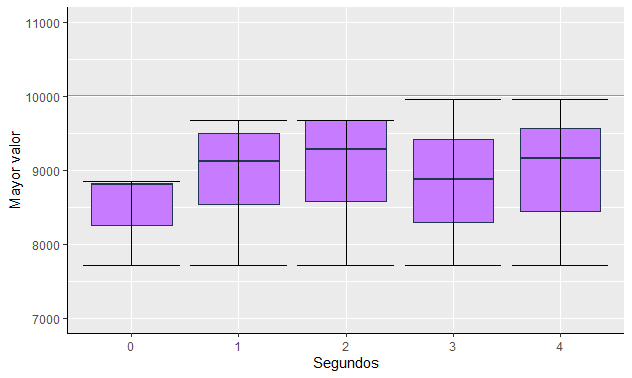
\includegraphics[width=\linewidth]{r1pob30.png}
\caption{30}
\label{bp1}
\end{subfigure}
\begin{subfigure}[b]{0.3\linewidth}
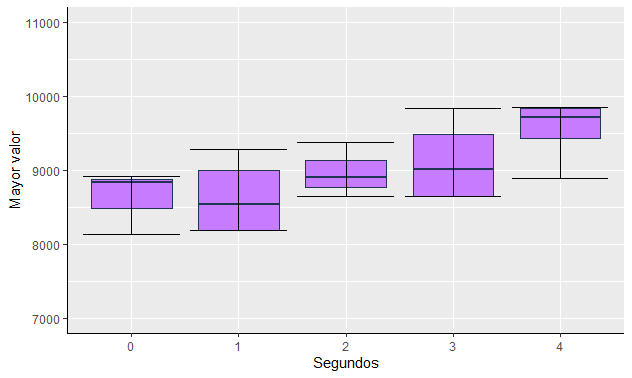
\includegraphics[width=\linewidth]{r1pob40.png}
\caption{40}
\label{cp1}
\end{subfigure}
\label{fig3}
\end{figure}

Con estas gráficas se procedió a hacer el análisis estadístico con Shapiro–Wilk \cite{shapiro} y Wilcox \cite{pairwise}.

\begin{lstlisting} [language=R, caption= Código para gráficas y análisis estadístico.]

#Mutaciones
library(ggplot2)
datos$segundo = as.factor(datos$segundo)
datoss = split.data.frame(datos, f = datos$pm)

ggplot(datoss$`0.05`, aes(x= segundo, y= mejor)) + 
  geom_boxplot(fill = "#F8766D", colour = "#1F3552")+
  stat_boxplot(geom = "errorbar", width = 0.9)+
  theme(axis.line = element_line(colour = "black", size = 0.25))+
  geom_hline(aes(yintercept=Optimo), colour="green")+
  labs(x = "Segundos", y = "Mayor valor")+
  coord_cartesian(ylim = c(7000, 10500))

ggplot(datoss$`0.1`, aes(x= segundo, y= mejor)) + 
  geom_boxplot(fill = "#F8766D", colour = "#1F3552")+
  stat_boxplot(geom = "errorbar", width = 0.9)+
  geom_hline(aes(yintercept=Optimo), colour="green")+
  theme(axis.line = element_line(colour = "black", size = 0.25))+
  labs(x = "Segundos", y = "Mayor valor")+
  coord_cartesian(ylim = c(7000, 10500))

ggplot(datoss$`0.5`, aes(x= segundo, y= mejor)) + 
  geom_boxplot(fill = "#F8766D", colour = "#1F3552")+
  stat_boxplot(geom = "errorbar", width = 0.9)+
  geom_hline(aes(yintercept=Optimo), colour="green")+
  theme(axis.line = element_line(colour = "black", size = 0.25))+
  labs(x = "Segundos", y = "Mayor valor")+
  coord_cartesian(ylim = c(7000, 10500))

cshapiro<-tapply(datos$mejor, datos$segundo, shapiro.test)

cwilcox<-pairwise.wilcox.test(datos$mejor, datos$segundo)

#cruzamientos
library(ggplot2)
datos$segundo = as.factor(datos$segundo)
datoss = split.data.frame(datos, f = datos$cruzamientos)

ggplot(datoss$`10`, aes(x= segundo, y= mejor)) + 
  geom_boxplot(fill = "#7CAE00", colour = "#1F3552")+
  stat_boxplot(geom = "errorbar", width = 0.9)+
  theme(axis.line = element_line(colour = "black", size = 0.25))+
  geom_hline(aes(yintercept=Optimo), colour="green")+
  labs(x = "Segundos", y = "Mayor valor")+
  coord_cartesian(ylim = c(6500, 10000))

ggplot(datoss$`20`, aes(x= segundo, y= mejor)) + 
  geom_boxplot(fill = "#7CAE00", colour = "#1F3552")+
  stat_boxplot(geom = "errorbar", width = 0.9)+
  geom_hline(aes(yintercept=Optimo), colour="green")+
  theme(axis.line = element_line(colour = "black", size = 0.25))+
  labs(x = "Segundos", y = "Mayor valor")+
  coord_cartesian(ylim = c(6500, 10000))

ggplot(datoss$`30`, aes(x= segundo, y= mejor)) + 
  geom_boxplot(fill = "#7CAE00", colour = "#1F3552")+
  stat_boxplot(geom = "errorbar", width = 0.9)+
  geom_hline(aes(yintercept=Optimo), colour="green")+
  theme(axis.line = element_line(colour = "black", size = 0.25))+
  labs(x = "Segundos", y = "Mayor valor")+
  coord_cartesian(ylim = c(6500, 10000))

cshapiro<-tapply(datos$mejor, datos$segundo, shapiro.test)

cwilcox<-pairwise.wilcox.test(datos$mejor, datos$segundo)

#poblacion

library(ggplot2)
datos$segundo = as.factor(datos$segundo)
datoss = split.data.frame(datos, f = datos$poblacion)

ggplot(datoss$`20`, aes(x= segundo, y= mejor)) + 
  geom_boxplot(fill = "#C77CFF", colour = "#1F3552")+
  stat_boxplot(geom = "errorbar", width = 0.9)+
  theme(axis.line = element_line(colour = "black", size = 0.25))+
  geom_hline(aes(yintercept=Optimo), colour="green")+
  labs(x = "Segundos", y = "Mayor valor")+
  coord_cartesian(ylim = c(7000, 11000))

ggplot(datoss$`30`, aes(x= segundo, y= mejor)) + 
  geom_boxplot(fill = "#C77CFF", colour = "#1F3552")+
  stat_boxplot(geom = "errorbar", width = 0.9)+
  geom_hline(aes(yintercept=Optimo), colour="green")+
  theme(axis.line = element_line(colour = "black", size = 0.25))+
  labs(x = "Segundos", y = "Mayor valor")+
  coord_cartesian(ylim = c(7000, 11000))

ggplot(datoss$`40`, aes(x= segundo, y= mejor)) + 
  geom_boxplot(fill = "#C77CFF", colour = "#1F3552")+
  stat_boxplot(geom = "errorbar", width = 0.9)+
  geom_hline(aes(yintercept=Optimo), colour="green")+
  theme(axis.line = element_line(colour = "black", size = 0.25))+
  labs(x = "Segundos", y = "Mayor valor")+
  coord_cartesian(ylim = c(7000, 11000))


cshapiro<-tapply(datos$mejor, datos$segundo, shapiro.test)

cwilcox<-pairwise.wilcox.test(datos$mejor, datos$segundo)
\end{lstlisting}

\begin{table}[h!]
\centering
\caption{Resultados de la prueba Shapiro–Wilk para la regla 1 en probabilidad de mutaciones.}
\label{tabla2}
\begin{tabular}{|c|r|r|}
\hline
seg & \multicolumn{1}{c|}{W} & \multicolumn{1}{c|}{P} \\ \hline
0 & 0.8388 & 0.0561 \\ \hline
1 & 0.9136 & 0.0997 \\ \hline
2 & 0.9590 & 0.6753 \\ \hline
3 & 0.9397 & 0.3796 \\ \hline
4 & 0.9425 & 0.4901 \\ \hline
\end{tabular}
\end{table}

\begin{table}[h!]
\centering
\caption{Resultados de la prueba Shapiro–Wilk para la regla 1 en cruzamiento.}
\label{tabla3}
\begin{tabular}{|c|r|r|}
\hline
seg & \multicolumn{1}{c|}{W} & \multicolumn{1}{c|}{P} \\ \hline
0 & 0.8510 & 0.0765 \\ \hline
1 & 0.8317 & 0.0246 \\ \hline
2 & 0.8289 & 0.0434 \\ \hline
3 & 0.8300 & 0.0446 \\ \hline
4 & 0.8851 & 0.1207 \\ \hline
\end{tabular}
\end{table}

\begin{table}[h!]
\centering
\caption{Resultados de la prueba Shapiro–Wilk para la regla 1 en población.}
\label{tabla4}
\begin{tabular}{|c|r|r|}
\hline
seg & \multicolumn{1}{c|}{W} & \multicolumn{1}{c|}{P} \\ \hline
0 & 0.9478 & 0.6668 \\ \hline
1 & 0.9170 & 0.1992 \\ \hline
2 & 0.9616 & 0.7495 \\ \hline
3 & 0.9169 & 0.2617 \\ \hline
4 & 0.8706 & 0.0534 \\ \hline
\end{tabular}
\end{table}

\begin{table}[h!]
\centering
\caption{Resultados de la prueba por parejas de Wilcox para la regla 1 en probabilidad de mutaciones.}
\label{tabla5}
\begin{tabular}{|c|l|l|c|c|}
\hline
seg & \multicolumn{1}{c|}{0} & \multicolumn{1}{c|}{1} & 2 & 3 \\ \hline
1 & 0.4864 & \multicolumn{1}{c|}{-} & - & - \\ \hline
2 & 0.2127 & 0.2127 & - & - \\ \hline
3 & 0.0608 & 0.0214 & \multicolumn{1}{l|}{0.4740} & - \\ \hline
4 & 0.0120 & 0.0025 & \multicolumn{1}{l|}{0.0992} & \multicolumn{1}{l|}{0.4740} \\ \hline
\end{tabular}
\end{table}

\begin{table}[h!]
\centering
\caption{Resultados de la prueba por parejas de Wilcox para la regla 1 en cruzamientos.}
\label{tabla6}
\begin{tabular}{|c|r|r|c|c|}
\hline
seg & \multicolumn{1}{c|}{0} & \multicolumn{1}{c|}{1} & 2 & 3 \\ \hline
1 & 1.00 & \multicolumn{1}{c|}{-} & - & - \\ \hline
2 & 1.00 & 1.00 & - & - \\ \hline
3 & 0.74 & 0.46 & \multicolumn{1}{r|}{0.46} & - \\ \hline
4 & 1.00 & 0.74 & \multicolumn{1}{r|}{0.74} & \multicolumn{1}{r|}{1.00} \\ \hline
\end{tabular}
\end{table}

\newpage

\begin{table}[h!]
\centering
\caption{Resultados de la prueba por parejas de Wilcox para la regla 1 en población.}
\label{tabla7}
\begin{tabular}{|c|r|r|c|c|}
\hline
seg & \multicolumn{1}{c|}{0} & \multicolumn{1}{c|}{1} & 2 & 3 \\ \hline
1 & 0.926 & \multicolumn{1}{c|}{-} & - & - \\ \hline
2 & 0.313 & 0.926 & - & - \\ \hline
3 & 0.313 & 0.823 & \multicolumn{1}{r|}{0.926} & - \\ \hline
4 & 0.037 & 0.137 & \multicolumn{1}{r|}{0.793} & \multicolumn{1}{r|}{0.926} \\ \hline
\end{tabular}
\end{table}

Del mismo modo se hizo para la regla 2.

\begin{figure}[h!]
\centering
\caption{Variación de probabilidad de mutación para la regla 2.}
\begin{subfigure}[b]{0.3\linewidth}
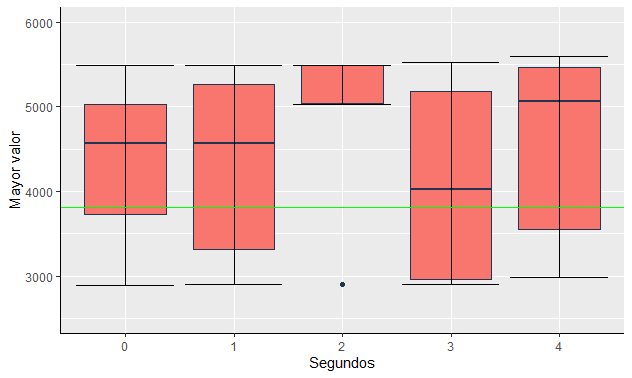
\includegraphics[width=\linewidth]{r2pm0.05.png}
\caption{0.05}
\label{am2}
\end{subfigure}
\begin{subfigure}[b]{0.3\linewidth}
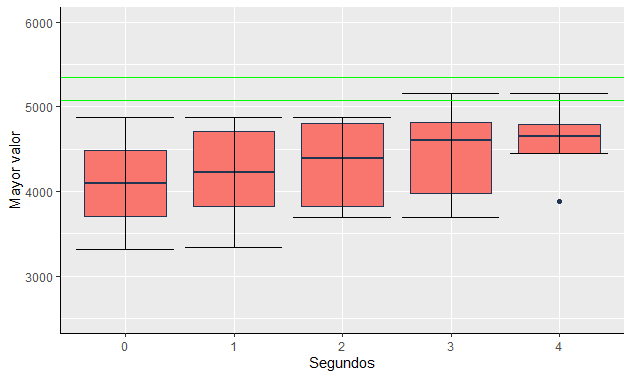
\includegraphics[width=\linewidth]{r2pm0.1.png}
\caption{0.1}
\label{bm2}
\end{subfigure}
\begin{subfigure}[b]{0.3\linewidth}
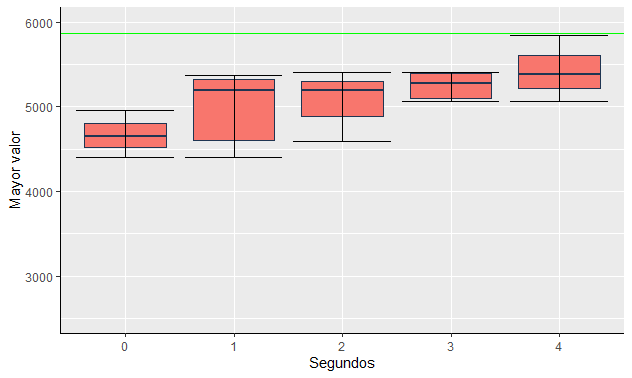
\includegraphics[width=\linewidth]{r2pm0.5.png}
\caption{0.5}
\label{cm2}
\end{subfigure}
\label{fig4}
\end{figure}

\begin{figure}[h!]
\centering
\caption{Variación de cruzamientos para la regla 2.}
\begin{subfigure}[b]{0.3\linewidth}
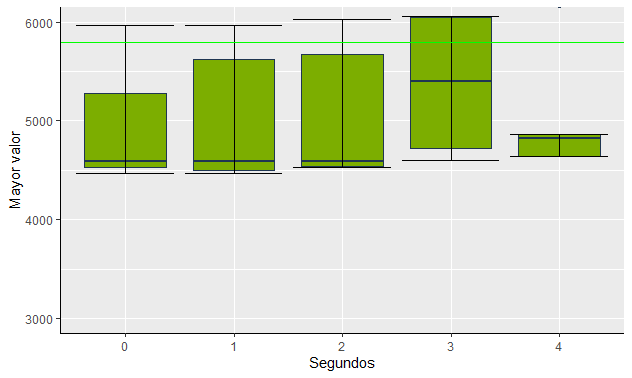
\includegraphics[width=\linewidth]{r2rep10.png}
\caption{10}
\label{ac2}
\end{subfigure}
\begin{subfigure}[b]{0.3\linewidth}
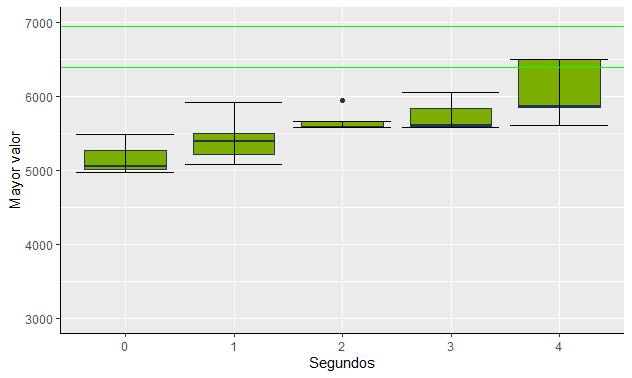
\includegraphics[width=\linewidth]{r2rep20.png}
\caption{20}
\label{bc2}
\end{subfigure}
\begin{subfigure}[b]{0.3\linewidth}
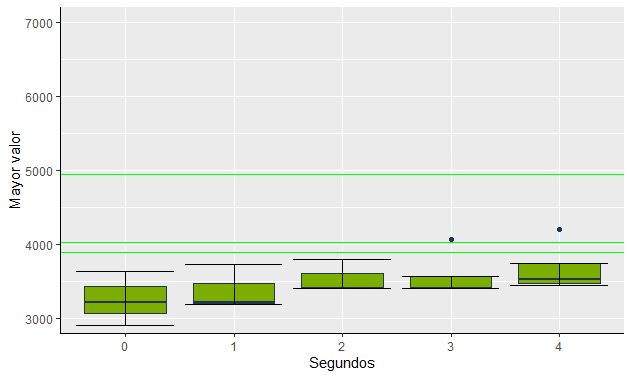
\includegraphics[width=\linewidth]{r2rep30.png}
\caption{30}
\label{cc2}
\end{subfigure}
\label{fig5}
\end{figure}

\begin{figure}[h!]
\centering
\caption{Variación de población para regla 2.}
\begin{subfigure}[b]{0.3\linewidth}
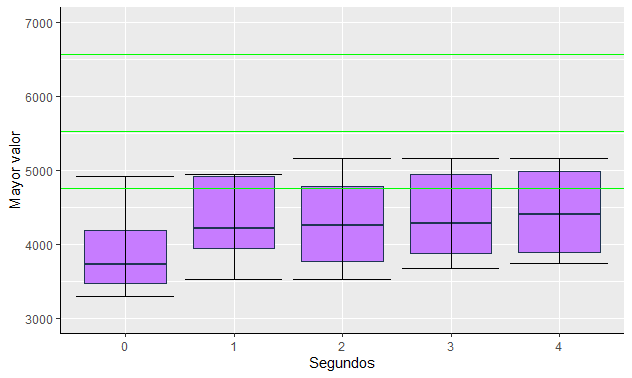
\includegraphics[width=\linewidth]{r2pob20.png}
\caption{20}
\label{ap2}
\end{subfigure}
\begin{subfigure}[b]{0.3\linewidth}
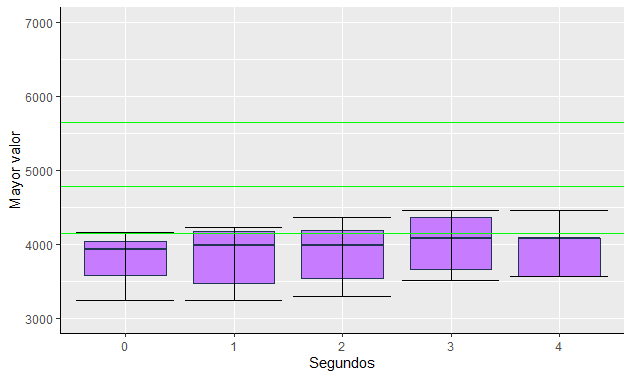
\includegraphics[width=\linewidth]{r2pob30.png}
\caption{30}
\label{bp2}
\end{subfigure}
\begin{subfigure}[b]{0.3\linewidth}
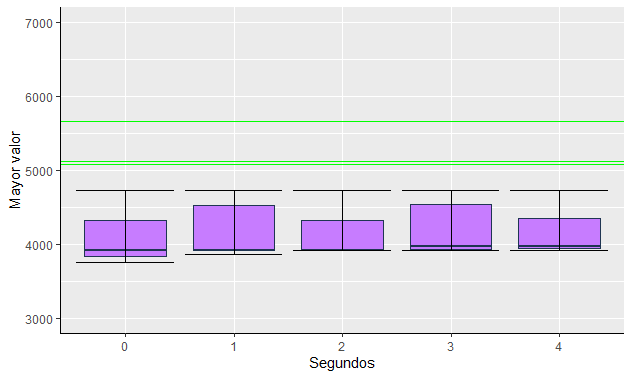
\includegraphics[width=\linewidth]{r2pob40.png}
\caption{40}
\label{cp2}
\end{subfigure}
\label{fig6}
\end{figure}

\begin{table}[h!]
\centering
\caption{Resultados de la prueba Shapiro–Wilk para la regla 2 en probabilidad de mutaciones.}
\label{tabla8}
\begin{tabular}{|c|r|r|}
\hline
seg & \multicolumn{1}{c|}{W} & \multicolumn{1}{c|}{P} \\ \hline
0 & 0.9393 & 0.5754 \\ \hline
1 & 0.9062 & 0.0738 \\ \hline
2 & 0.9003 & 0.1141 \\ \hline
3 & 0.8231 & 0.0056 \\ \hline
4 & 0.8596 & 0.0380 \\ \hline
\end{tabular}
\end{table}

\newpage

\begin{table}[h!]
\centering
\caption{Resultados de la prueba Shapiro–Wilk para la regla 2 en cruzamiento.}
\label{tabla9}
\begin{tabular}{|c|r|r|}
\hline
seg & \multicolumn{1}{c|}{W} & \multicolumn{1}{c|}{P} \\ \hline
0 & 0.9565 & 0.7612 \\ \hline
1 & 0.9188 & 0.2116 \\ \hline
2 & 0.8860 & 0.0861 \\ \hline
3 & 0.8531 & 0.0469 \\ \hline
4 & 0.9203 & 0.2222 \\ \hline
\end{tabular}
\end{table}

\begin{table}[h!]
\centering
\caption{Resultados de la prueba Shapiro–Wilk para la regla 2 en población.}
\label{tabla10}
\begin{tabular}{|c|l|l|}
\hline
seg & \multicolumn{1}{c|}{W} & \multicolumn{1}{c|}{P} \\ \hline
0 & 0.9271 & 0.4201 \\ \hline
1 & 0.9299 & 0.2169 \\ \hline
2 & 0.9603 & 0.6983 \\ \hline
3 & 0.9379 & 0.2677 \\ \hline
4 & 0.9176 & 0.2033 \\ \hline
\end{tabular}
\end{table}

\begin{table}[h!]
\centering
\caption{Resultados de la prueba por parejas de Wilcox para la regla 2 en probabilidad de mutaciones.}
\label{tabla11}
\begin{tabular}{|c|r|r|c|c|}
\hline
seg & \multicolumn{1}{c|}{0} & \multicolumn{1}{c|}{1} & 2 & 3 \\ \hline
1 & 1 & \multicolumn{1}{c|}{-} & - & - \\ \hline
2 & 1 & 1 & - & - \\ \hline
3 & 1 & 1 & \multicolumn{1}{r|}{1} & - \\ \hline
4 & 1 & 1 & \multicolumn{1}{r|}{1} & \multicolumn{1}{r|}{1} \\ \hline
\end{tabular}
\end{table}

\begin{table}[h!]
\centering
\caption{Resultados de la prueba por parejas de Wilcox para la regla 2 en cruzamientos.}
\label{tabla12}
\begin{tabular}{|c|r|r|c|c|}
\hline
seg & \multicolumn{1}{c|}{0} & \multicolumn{1}{c|}{1} & 2 & 3 \\ \hline
1 & 1 & \multicolumn{1}{c|}{-} & - & - \\ \hline
2 & 1 & 1 & - & - \\ \hline
3 & 1 & 1 & \multicolumn{1}{r|}{1} & - \\ \hline
4 & 1 & 1 & \multicolumn{1}{r|}{1} & \multicolumn{1}{r|}{1} \\ \hline
\end{tabular}
\end{table}

\begin{table}[h!]
\centering
\caption{Resultados de la prueba por parejas de Wilcox para la regla 2 en población.}
\label{tabla13}
\begin{tabular}{|c|r|r|c|c|}
\hline
seg & \multicolumn{1}{c|}{0} & \multicolumn{1}{c|}{1} & 2 & 3 \\ \hline
1 & 1 & \multicolumn{1}{c|}{-} & - & - \\ \hline
2 & 1 & 1 & - & - \\ \hline
3 & 1 & 1 & \multicolumn{1}{r|}{1} & - \\ \hline
4 & 1 & 1 & \multicolumn{1}{r|}{1} & \multicolumn{1}{r|}{1} \\ \hline
\end{tabular}
\end{table}

\newpage

Y de igual forma para la regla 3.

\begin{figure}[h!]
\centering
\caption{Variación de probabilidad de mutación para la regla 3.}
\begin{subfigure}[b]{0.3\linewidth}
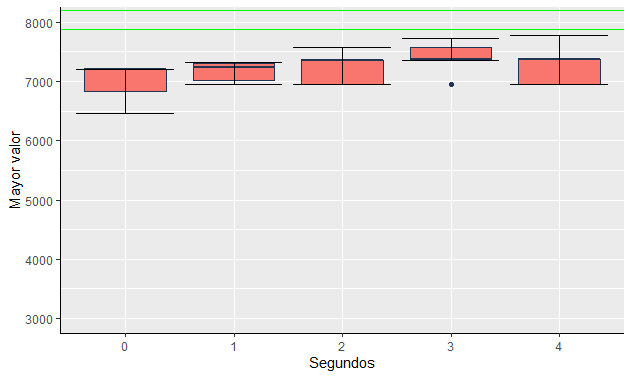
\includegraphics[width=\linewidth]{r3pm0.05.png}
\caption{0.05}
\label{am3}
\end{subfigure}
\begin{subfigure}[b]{0.3\linewidth}
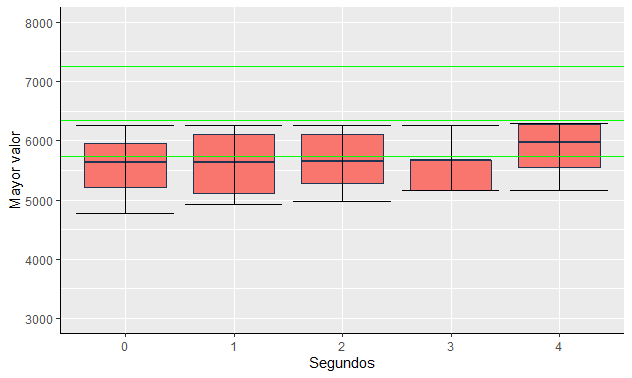
\includegraphics[width=\linewidth]{r3pm0.1.png}
\caption{0.1}
\label{bm3}
\end{subfigure}
\begin{subfigure}[b]{0.3\linewidth}
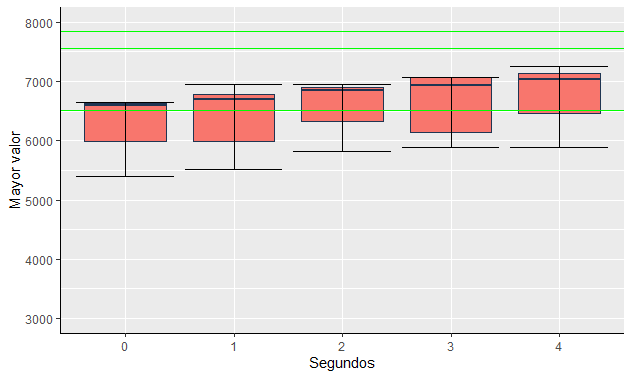
\includegraphics[width=\linewidth]{r3pm0.5.png}
\caption{0.5}
\label{cm3}
\end{subfigure}
\label{fig7}
\end{figure}

\begin{figure}[h!]
\centering
\caption{Variación de cruzamientos para la regla 3.}
\begin{subfigure}[b]{0.3\linewidth}
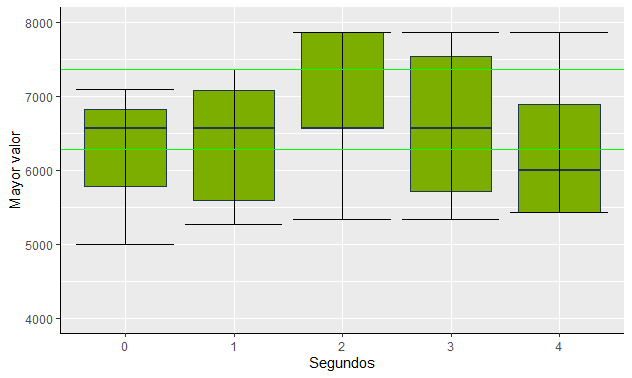
\includegraphics[width=\linewidth]{r3rep10.png}
\caption{10}
\label{ac3}
\end{subfigure}
\begin{subfigure}[b]{0.3\linewidth}
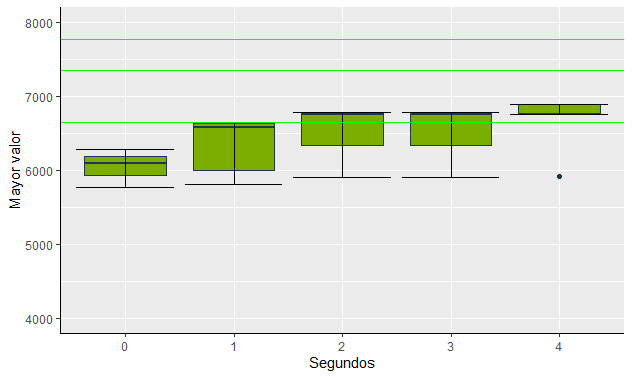
\includegraphics[width=\linewidth]{r3rep20.png}
\caption{20}
\label{bc3}
\end{subfigure}
\begin{subfigure}[b]{0.3\linewidth}
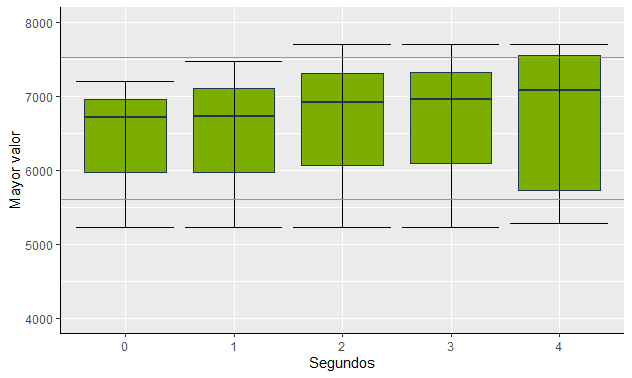
\includegraphics[width=\linewidth]{r3rep30.png}
\caption{30}
\label{cc3}
\end{subfigure}
\label{fig8}
\end{figure}

\begin{figure}[h!]
\centering
\caption{Variación de población para regla 3.}
\begin{subfigure}[b]{0.3\linewidth}
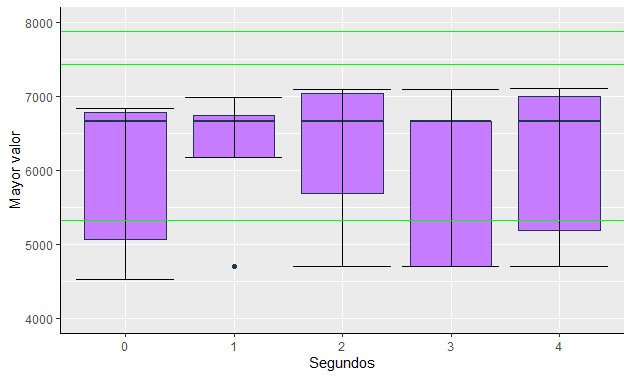
\includegraphics[width=\linewidth]{r3pob20.png}
\caption{20}
\label{ap3}
\end{subfigure}
\begin{subfigure}[b]{0.3\linewidth}
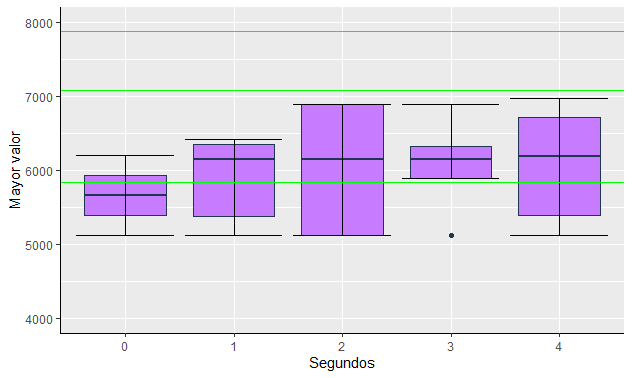
\includegraphics[width=\linewidth]{r3pob30.png}
\caption{30}
\label{bp3}
\end{subfigure}
\begin{subfigure}[b]{0.3\linewidth}
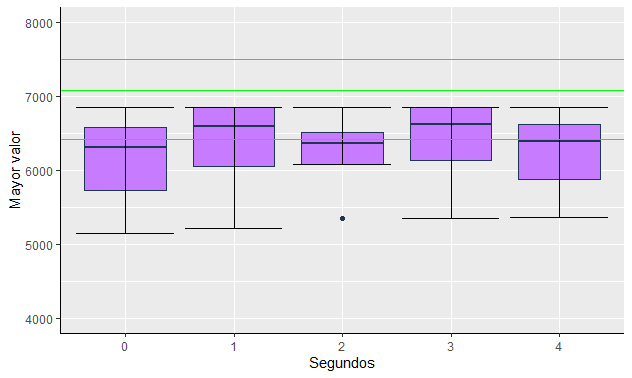
\includegraphics[width=\linewidth]{r3pob40.png}
\caption{40}
\label{cp3}
\end{subfigure}
\label{fig9}
\end{figure}

\begin{table}[h!]
\centering
\caption{Resultados de la prueba Shapiro–Wilk para la regla 3 en probabilidad de mutaciones.}
\label{tabla14}
\begin{tabular}{|c|r|r|}
\hline
seg & \multicolumn{1}{c|}{W} & \multicolumn{1}{c|}{P} \\ \hline
0 & 0.9335 & 0.5156 \\ \hline
1 & 0.8953 & 0.0476 \\ \hline
2 & 0.9286 & 0.2916 \\ \hline
3 & 0.9095 & 0.1143 \\ \hline
4 & 0.9409 & 0.5107 \\ \hline
\end{tabular}
\end{table}

\newpage

\begin{table}[h!]
\centering
\caption{Resultados de la prueba Shapiro–Wilk para la regla 3 en cruzamiento.}
\label{tabla15}
\begin{tabular}{|c|r|r|}
\hline
seg & \multicolumn{1}{c|}{W} & \multicolumn{1}{c|}{P} \\ \hline
0 & 0.9504 & 0.6947 \\ \hline
1 & 0.8964 & 0.0838 \\ \hline
2 & 0.9165 & 0.2907 \\ \hline
3 & 0.9128 & 0.2321 \\ \hline
4 & 0.8991 & 0.0922 \\ \hline
\end{tabular}
\end{table}

\begin{table}[h!]
\centering
\caption{Resultados de la prueba Shapiro–Wilk para la regla 3 en población.}
\label{tabla16}
\begin{tabular}{|c|r|r|}
\hline
seg & \multicolumn{1}{c|}{W} & \multicolumn{1}{c|}{P} \\ \hline
0 & 0.8532 & 0.0402 \\ \hline
1 & 0.8689 & 0.0405 \\ \hline
2 & 0.8432 & 0.0108 \\ \hline
3 & 0.8627 & 0.0418 \\ \hline
4 & 0.8647 & 0.0282 \\ \hline
\end{tabular}
\end{table}

\begin{table}[h!]
\centering
\caption{Resultados de la prueba por parejas de Wilcox para la regla 3 en probabilidad de mutaciones.}
\label{tabla17}
\begin{tabular}{|c|r|r|c|c|}
\hline
seg & \multicolumn{1}{c|}{0} & \multicolumn{1}{c|}{1} & 2 & 3 \\ \hline
1 & 1 & \multicolumn{1}{c|}{-} & - & - \\ \hline
2 & 1 & 1 & - & - \\ \hline
3 & 1 & 1 & \multicolumn{1}{r|}{1} & - \\ \hline
4 & 1 & 1 & \multicolumn{1}{r|}{1} & \multicolumn{1}{r|}{1} \\ \hline
\end{tabular}
\end{table}

\begin{table}[h!]
\centering
\caption{Resultados de la prueba por parejas de Wilcox para la regla 3 en cruzamientos.}
\label{tabla18}
\begin{tabular}{|c|r|r|c|c|}
\hline
seg & \multicolumn{1}{c|}{0} & \multicolumn{1}{c|}{1} & 2 & 3 \\ \hline
1 & 1 & \multicolumn{1}{c|}{-} & - & - \\ \hline
2 & 1 & 1 & - & - \\ \hline
3 & 1 & 1 & \multicolumn{1}{r|}{1} & - \\ \hline
4 & 1 & 1 & \multicolumn{1}{r|}{1} & \multicolumn{1}{r|}{1} \\ \hline
\end{tabular}
\end{table}

\begin{table}[h!]
\centering
\caption{Resultados de la prueba por parejas de Wilcox para la regla 3 en población.}
\label{tabla19}
\begin{tabular}{|c|r|r|c|c|}
\hline
seg & \multicolumn{1}{c|}{0} & \multicolumn{1}{c|}{1} & 2 & 3 \\ \hline
1 & 1 & \multicolumn{1}{c|}{-} & - & - \\ \hline
2 & 1 & 1 & - & - \\ \hline
3 & 1 & 1 & \multicolumn{1}{r|}{1} & - \\ \hline
4 & 1 & 1 & \multicolumn{1}{r|}{1} & \multicolumn{1}{r|}{1} \\ \hline
\end{tabular}
\end{table}

Todos los códigos para la generación del presente trabajo se encuentran en mi github \cite{eduardo}.

\section{Conclusiones}
De la regla 1 podemos concluir que tiende a llegar al óptimo conforme más tiempo pase para las 3 instancias, la que menos valor mayor alcanzó fué con los cruzamientos junto con valores óptimos bajos, que también fué la que no presentó normalidad. De la prueba de Wilcox para la regla 1 se tienen diferencias entre el primer y último segundo para la probabilidad de mutaciones y fué el que presentó mayores diferencias entre grupos. La que mantuvo valores mayores fué la variación de población.

De la regla 2 podemos concluir que igual tiende a llegar al óptimo conforme más tiempo pase. La que menos valor mayor alcanzó en general fué con la población. Siendo la de cruzamientos a 30 la menor de todas y la de 20 la mayor de todas. En su mayoría presentaron normalidad y no se observaron diferencias entre grupos.

De la regla 3 podemos concluir que igual se observa una tendencia para la probabilidad de mutación a alcanzar un mayor valor. Siendo que los otros se quedan relativamente igual entre ellos. El mayor valor lo alcanzó la variación de cruzamientos. La variación de población fué la que no presentó normalidad y obtuvo valores bajos. En los 3 no se apreciaron diferencias entre grupos.

En general el mayor valor alcanzado regla 1 a 20 de población, menor valor alcanzado regla 2 a 30 de cruzamientos, más óptimos cercanos para la variación de cruzamiento.


\bibliography{referencias}
\bibliographystyle{plainnat}
\end{document}
